\documentclass[12pt,reqno,oneside]{amsart}
\usepackage{import}
%===============================%
%  Packages and basic settings  %
%===============================%
\usepackage[headheight=15pt,rmargin=0.5in,lmargin=0.5in,tmargin=0.75in,bmargin=0.75in]{geometry}
\usepackage{imakeidx}
\usepackage{framed}
\usepackage{amssymb}
\usepackage{amsmath}
\usepackage{mathrsfs}
\usepackage{enumitem}
\usepackage{hyperref}
\usepackage{appendix}
\usepackage[capitalise,noabbrev]{cleveref}
\usepackage{tikz}
\usepackage{tikz-cd}
\usepackage{nomencl}\makenomenclature
\usetikzlibrary{braids,arrows,decorations.markings,calc}

%====================================%
%  Theorems, environments & cleveref  %
%====================================%
\newtheorem{theorem}{Theorem}[section]
\newtheorem{proposition}{Proposition}[section]
\newtheorem{corollary}{Corollary}[section]
\newtheorem{lemma}{Lemma}[section]
\newtheorem{conjecture}{Conjecture}[section]
\newtheorem{remark}{Remark}[section]

\newenvironment{stabular}[2][1]
  {\def\arraystretch{#1}\tabular{#2}}
  {\endtabular}

%==================================%
%  Custom commands & environments  %
%==================================%
\newcommand{\legendre}[2]{\left(\frac{#1}{#2}\right)}
\newcommand{\dlegendre}[2]{\displaystyle{\left(\frac{#1}{#2}\right)}}
\newcommand{\tlegendre}[2]{\textstyle{\left(\frac{#1}{#2}\right)}}
\newcommand{\psum}{\sideset{}{'}\sum}
\newcommand{\asum}{\sideset{}{^{\ast}}\sum}
\newcommand{\tmod}[1]{\ \left(\text{mod }#1\right)}
\newcommand{\xto}[1]{\xrightarrow{#1}}
\newcommand{\xfrom}[1]{\xleftarrow{#1}}
\newcommand{\normal}{\mathrel{\unlhd}}
\newcommand{\mf}{\mathfrak}
\newcommand{\mc}{\mathcal}
\newcommand{\ms}{\mathscr}

\newcommand{\Mat}{\mathrm{Mat}}
\newcommand{\GL}{\mathrm{GL}}
\newcommand{\SL}{\mathrm{SL}}
\newcommand{\PSL}{\mathrm{PSL}}
\renewcommand{\O}{\mathrm{O}}
\newcommand{\SO}{\mathrm{SO}}
\newcommand{\U}{\mathrm{U}}
\newcommand{\Sp}{\mathrm{Sp}}

\newcommand{\N}{\mathbb{N}}
\newcommand{\Z}{\mathbb{Z}}
\newcommand{\Q}{\mathbb{Q}}
\newcommand{\R}{\mathbb{R}}
\newcommand{\C}{\mathbb{C}}
\newcommand{\F}{\mathbb{F}}
\renewcommand{\H}{\mathbb{H}}
\renewcommand{\P}{\mathbb{P}}

\renewcommand{\a}{\alpha}
\renewcommand{\b}{\beta}
\newcommand{\g}{\gamma}
\renewcommand{\d}{\delta}
\newcommand{\z}{\zeta}
\renewcommand{\t}{\theta}
\renewcommand{\i}{\iota}
\renewcommand{\k}{\kappa}
\renewcommand{\l}{\lambda}
\newcommand{\s}{\sigma}
\newcommand{\w}{\omega}

\newcommand{\G}{\Gamma}
\newcommand{\D}{\Delta}
\renewcommand{\L}{\Lambda}
\newcommand{\W}{\Omega}

\newcommand{\e}{\varepsilon}
\newcommand{\vt}{\vartheta}
\newcommand{\vphi}{\varphi}
\newcommand{\emt}{\varnothing}

\newcommand{\x}{\times}
\newcommand{\ox}{\otimes}
\newcommand{\op}{\oplus}
\newcommand{\bigox}{\bigotimes}
\newcommand{\bigop}{\bigoplus}
\newcommand{\del}{\partial}
\newcommand{\<}{\langle}
\renewcommand{\>}{\rangle}
\newcommand{\lf}{\lfloor}
\newcommand{\rf}{\rfloor}
\newcommand{\wtilde}{\widetilde}
\newcommand{\what}{\widehat}
\newcommand{\conj}{\overline}
\newcommand{\cchi}{\conj{\chi}}

\DeclareMathOperator{\id}{\textrm{id}}
\DeclareMathOperator{\sgn}{\mathrm{sgn}}
\DeclareMathOperator{\im}{\mathrm{im}}
\DeclareMathOperator{\rk}{\mathrm{rk}}
\DeclareMathOperator{\tr}{\mathrm{trace}}
\DeclareMathOperator{\nm}{\mathrm{norm}}
\DeclareMathOperator{\ord}{\mathrm{ord}}
\DeclareMathOperator{\Hom}{\mathrm{Hom}}
\DeclareMathOperator{\End}{\mathrm{End}}
\DeclareMathOperator{\Aut}{\mathrm{Aut}}
\DeclareMathOperator{\Tor}{\mathrm{Tor}}
\DeclareMathOperator{\Ann}{\mathrm{Ann}}
\DeclareMathOperator{\Gal}{\mathrm{Gal}}
\DeclareMathOperator{\Trace}{\mathrm{Trace}}
\DeclareMathOperator{\Norm}{\mathrm{Norm}}
\DeclareMathOperator{\Span}{\mathrm{Span}}
\DeclareMathOperator*{\Res}{\mathrm{Res}}
\DeclareMathOperator{\Vol}{\mathrm{Vol}}
\DeclareMathOperator{\Li}{\mathrm{Li}}
\renewcommand{\Re}{\mathrm{Re}}
\renewcommand{\Im}{\mathrm{Im}}

\newcommand{\GH}{\G\backslash\H}
\newcommand{\GG}{\G_{\infty}\backslash\G}

\newenvironment{psmallmatrix}
  {\left(\begin{smallmatrix}}
  {\end{smallmatrix}\right)}

%============%
%  Comments  %
%============%
\newcommand{\todo}[1]{\textcolor{red}{\sf Todo: [#1]}}

%===================%
%  Label reminders  %
%===================%
% [label=(\roman*)]
% [label=(\alph*)]
% [label=(\arabic{enumi})]

%==================%
%  Other settings  %
%==================%
\pgfdeclarelayer{background}
\pgfsetlayers{background,main}
\tikzset{->-/.style={decoration={
  markings,
  mark=at position .5 with {\arrow{>}}},postaction={decorate}}}

%=================%
%  Title & Index  %
%=================%
\title{A root systems primer}
\author{Henry Twiss}
\date{2024}
\makeindex

\begin{document}

\begin{abstract}
    We present an axiomatic introduction to finite root systems and their classification via Dynkin diagrmas. Much of the information discussed here is a more detailed presentation of the root systems chapter in \cite{humphreys1972introduction}. For a discussion about how root systems arise as sets of generalized eigenvectors decomposing Lie algebras see \cite{humphreys1972introduction}.
\end{abstract}

\maketitle

\section{Euclidean Vector Spaces}
    Throughout let $V$ be a finite-dimensional Euclidean vector space. That is, $V$ is a finite-dimension vector space over $\R$ endowed with a positive definite symmetric blinear form $(\cdot,\cdot)$. A \textbf{hyperplane} in $V$ is an subspace of codimension $1$. A \textbf{reflection} in $V$ is a invertible linear transformation that fixes some hyperplane and sends any vector orthogonal to that hyperplane to its negative. Clearly reflections are orthogonal transformations ane hence are isometries. Moreover, $V$ has an induced norm $||\cdot|| = \sqrt{\<\cdot,\cdot\>}$ and this norm induces a natural metric topology on $V$ making $V$ a complete metric space. Any nonzero vector $v \in V$ determines its \textbf{reflecting hyperplane} $H_{v}$ defined by
    \[
        H_{v} = \{w \in V:(v,w) = 0\},
    \]
    which is the hyperplane orthogonal to $v$. We say that a vector $w \in V$ lies on the \textbf{positive side} of $H_{v}$ if $(v,w) > 0$ and on the \textbf{negative side} of $H_{v}$ if $(v,w) < 0$. Moreover, any vector proportional to $v$ determines the same reflecting hyperplane. Accordingly, let
    \[
        \s_{v}(w) = w-2\frac{(v,w)}{(v,v)}v, 
    \]
    be the reflection through the hyperplane $H_{v}$. This is indeed a reflection because if $w \in H_{v}$ then $\s_{v}(w) = w$ and $\s_{v}(v) = -v$. Recall that if $v,w \in V$ are orthogonal vectors, that is $(v,w) = 0$, then $\s_{v}\s_{w} = \s_{w}\s_{v}$. Also, if the angle between $v$ and $w$ is $\t$ then $\s_{v}\s_{w}$ is a rotation through angle $2\t$. Lastly, we define an operator $\<\cdot,\cdot\>:(V-\{\mathbf{0}\}) \x (V-\{\mathbf{0}\}) \to \R$ by
    \[
        \<w,v\> = 2\frac{(v,w)}{(v,v)},
    \]
    Note that $\<\cdot,\cdot\>$ is not an inner product as it need not be symmetric and is linear only in the first argument. However, we have the following simplified formula for the reflection $\s_{v}$:
    \[
        \s_{v}(w) = w-\<w,v\>v.
    \]
\section{Axiomatic Root Systems}
     A \textbf{root system} $\Phi$ in $E$, whose elements $\a \in \Phi$ are called \textbf{roots}, is a finite set of nonzero vectors that satisfty the following properties:

    \begin{enumerate}[label=(\roman*)]
        \item $\Phi$ is a spanning set for $V$.
        \item For any root $\a \in \Phi$, then the only scalar multiples of $\a$ that belong to $\Phi$ are $\a$ itself and $-\a$.
        \item For every root $\a \in \Phi$, $\Phi$ is closed under the reflection $\s_{\a}$.
        \item If $\a,\b \in \Phi$ are roots, then the projection of $\b$ onto the line through $\a$ is an integer or half-integer multiple of $\a$.
    \end{enumerate}

    The last two properties can be equivalently expressed in more algebraic forms:

    \begin{enumerate}[label=(\roman*)]
        \setcounter{enumi}{2}
        \item For any two roots $\a,\b \in \Phi$, $\Phi$ contains the element
        \[
            \s_{\a}(\b) = \b-2\frac{(\a,\b)}{(\a,\a)}\a = \b-\<\b,\a\>\a.
        \]
        \item If $\a,\b \in \Phi$ are roots, then the number $\<\b,\a\> = 2\frac{(\a,\b)}{(\a,\a)}$ is an integer.
    \end{enumerate}
    
    In particular, property (iv) means that $\<\cdot,\cdot\>$ restricted to $\Phi \x \Phi$ is a map of the form $\<\cdot,\cdot\>:\Phi \x \Phi \to \Z$ and so from property (iii) we see that $\s_{\a}$ just adds an integral multiple of $\a$ to $\b$. Sometimes authors omit property (ii) and (iv). In these cases, if (ii) is satisfied we say that the root system is \textbf{reduced} and if (iv) is satisfied we say that the root system is \textbf{crystallographic}. We define the \textbf{rank} of $\Phi$ to be the dimension of $V$. Throughout we will always assume our root systems are reduced and crystallographic (that is they satisfty (i)-(iv)) unless specified otherwise.

    The two simplest examples of root systems are the rank $2$ root systems of type $A_{1}$ and type $A_{2}$:

    \begin{center}
    \begin{tikzpicture}[scale=1.5]
        \draw[thick,-stealth](0,0) to (60:{sqrt(3)/2}) node [above right] {$\a+\b$};
        \draw[thick,-stealth](0,0) to (240:{sqrt(3)/2});
        \draw[thick,-stealth](0,0) to (180:{sqrt(3)/2});
        \draw[thick,-stealth](0,0) to (360:{sqrt(3)/2}) node [right] {$\a$};
        \draw[thick,-stealth] (0:0) to (120:{sqrt(3)/2}) node [above left] {$\b$};
        \draw[thick,-stealth] (0:0) to (300:{sqrt(3)/2});
        
        \draw[dotted,] (0:0) to (30:{sqrt(3)/2});
        \draw[dotted,] (0:0) to (30:{-sqrt(3)/2});
        \draw[dotted,] (0:0) to (90:{sqrt(3)/2});
        \draw[dotted,] (0:0) to (90:{-sqrt(3)/2});
        \draw[dotted,] (0:0) to (150:{sqrt(3)/2});
        \draw[dotted,] (0:0) to (150:{-sqrt(3)/2});

        \node at (0,-1.5) {$A_{2}$};
        
        \begin{scope}[shift = {(-4,0)}]
            \draw[thick,-stealth](0,0) to (180:{sqrt(3)/2});
            \draw[thick,-stealth](0,0) to (360:{sqrt(3)/2}) node [right] {$\a$};
            
            \draw[dotted,] (0:0) to (90:{sqrt(3)/2});
            \draw[dotted,] (0:0) to (90:{-sqrt(3)/2});

            \node at (0,-1.5) {$A_{1}$};
        \end{scope}
    \end{tikzpicture}
    \end{center}

    For these root systems, note that the dotted lines denote the reflections that the corresponding root system is invariant under. In particular, every dotted line is orthogonal to a pair of roots. The root system of type $A_{2}$ will be our running example in our discussion.

    Although we will not use them, we will describe dual root systems. Let $\Phi$ be a root system. For every $\a \in \Phi$ define the \textbf{dual root} $\a^{\vee}$ by
    \[
        \a^{\vee} = \frac{2\a}{(\a,\a)}.
    \]
    Then $\Phi^{\vee} = \{\a^{\vee}:\a \in \Phi\}$ is called the \textbf{dual} to $\Phi$. Clearly $\Phi^{\vee\vee} = \Phi$. Since the dual roots are just scalar multiples of the roots and
    \[
        \<\b^{\vee},\a^{\vee}\> = \left\<\frac{2\b}{(\b,\b)},\frac{2\a}{(\a,\a)}\right\> = \frac{2}{(\b,\b)}\left\<\b,\frac{2\a}{(\a,\a)}\right\> = \frac{4}{(\b,\b)}\frac{\left(\frac{2\a}{(\a,\a)},\b\right)}{\left(\frac{2\a}{(\a,\a)},\frac{2\a}{(\a,\a)}\right)} = 2\frac{(\b,\a)}{(\b,\b)} = \<\a,\b\>,
    \]
    $\Phi^{\vee}$ is also a root system.
\section{Pairs of Roots}
    It turns out that the angles between roots in a root system are quite restricted in general. This is a consequence of property (iv) which implies that $\<\b,\a\>$ and $\<\a,\b\>$ are integers. Without loss of generality we assume $\b \neq \pm \a$, equivalently $\a$ and $\b$ are non-proportional, and there is no additional harm in supposing $|\a| \le |\b|$. If $\t$ is the angle between $\a$ and $\b$, then
    \begin{align*}
        \<\b,\a\>\<\a,\b\> &= 4\frac{(\a,\b)}{(\a,\a)}\frac{(\b,\a)}{(\b,\b)} \\
        &= 4\frac{(\a,\b)^{2}}{|\a|^{2}|\b|^{2}} \\
        &= 4\cos^{2}(\t) \\
        &= (2\cos(\t))^{2},
    \end{align*}
    where in the third line we have made use of the formula $(\a,\b) = |\a||\b|\cos(\t)$. Since this is a square, we see that $\<\b,\a\>$ and $\<\a,\b\>$ must have the same sign. Moreover, since $(2\cos(\t))^{2}$ must be an integer and $2\cos(\t) \in [-2,2]$, we have $\<\b,\a\>\<\a,\b\> \in \{0,1,2,3,4\}$. As $\b \neq \pm \a$ we know $2\cos(\t) \neq \pm 2$ and so $\<\b,\a\>\<\a,\b\> \neq 4$. Combining these facts we see that the only possible values for $\t$ are those given in \cref{tab:root_angles}.

    \begin{table}[ht]
        \caption{}\label{tab:root_angles}
        \begin{stabular}[1.5]{|c|c|c|c|c|c|}
            \hline
            $\t$ & $\cos(\t)$ & $\<\b,\a\>$ & $\<\a,\b\>$ & $\frac{|\b|^{2}}{|\a|^{2}}$ \\
            \hline
            $\frac{\pi}{2}$ & $0$ & $0$ & $0$ & undetermined \\
            \hline
            $\frac{\pi}{3}$ & $\frac{1}{2}$ & $1$ & $1$ & $1$ \\
            \hline
            $\frac{2\pi}{3}$ & $-\frac{1}{2}$ & $-1$ & $-1$ & $1$ \\
            \hline
            $\frac{\pi}{4}$ & $\frac{\sqrt{2}}{2}$ & $2$ & $1$ & $2$ \\
            \hline
            $\frac{3\pi}{4}$ & $-\frac{\sqrt{2}}{2}$ & $-2$ & $-1$ & $2$ \\
            \hline
            $\frac{\pi}{6}$ & $\frac{\sqrt{3}}{2}$ & $3$ & $1$ & $3$ \\
            \hline
            $\frac{5\pi}{6}$ & $-\frac{\sqrt{3}}{2}$ & $-3$ & $-1$ & $3$ \\
            \hline
        \end{stabular}
    \end{table}

    In computing the table we have used the formulas $\<\b,\a\>\<\a,\b\> = (2\cos(\t))^{2}$, $\<\b,\a\> = 2\cos(\t)\frac{|\b|}{|\a|}$, and the assumption $|\a| \le |\b|$. Note that the condition $|\a| \le |\b|$ is only used in the last column to ensure that $\frac{|\b|^{2}}{|\a|^{2}}$ is an integer. Using this table we can prove a very useful lemma:

    \begin{lemma}\label{lem:sum_or_difference_is_a_root}
        Suppose $\a$ and $\b$ are non-proportional roots. If $(\a,\b) > 0$ then $\a-\b$ is a root. If $(\a,\b) < 0$ then $\a+\b$ is a root.
    \end{lemma}
    \begin{proof}
        If $(\a,\b) > 0$ then the angle between $\a$ and $\b$ is strictly acute so that $\cos(\t) > 0$. From \cref{tab:root_angles}, all of these cases correspond to either $\<\a,\b\> = 1$ or $\<\b,\a\> = 1$. If $\<\a,\b\> = 1$, then $\s_{\b}(\a) = \a-\b$ is a root and we are done. If $\<\b,\a\> = 1$, then $\s_{\a}(\b) = \b-\a$ is a root. But then $\s_{\b-\a}(\b-\a) = \a-\b$ is again a root. The second statement follows by using $-\b$ in place of $\b$.
    \end{proof}

    In particular, \cref{lem:sum_or_difference_is_a_root} states that one of $\a-\b$ or $\a+\b$ must be a root. For any two non-proportional roots $\a$ and $\b$, we define the \textbf{$\a$-root string through $\b$} (or simply \textbf{root string}) $S(\a,\b)$ to be the set of all roots of the form $\b+k\a$ for $k \in \Z$. In other words, $S(\a,\b) = \{\b+k\a:k \in \Z\} \cap \Phi $. We can describe this root string explicitely:

    \begin{proposition}\label{prop:sum_or_difference_is_a_root}
        For any two non-proportional roots $\a$ and $\b$, there exsits $u,v \in \Z_{\ge 0}$ such that
        \[
            S(\a,\b) = \{\b-u\a,\ldots,\b+v\a\},
        \]
        and $u-v = \<\b,\a\>$. 
    \end{proposition}
    \begin{proof}
        Let  $u,v \in \Z_{\ge 0}$ be the largest integers for which $\b+v\a \in \Phi$ and $\b-u\a \in \Phi$. Now suppose, by contradiction, that there exists some $k$ with $-u < k < v$ such that $\b+k\a \notin \Phi$. Then we can find integers $r$ and $q$ with $-u \le r < k < q \le v$ such that $\b+r\a \in \Phi$ and $\b+q\a \in \Phi$ but $\b+(r+1)\a \notin \Phi$ and $\b+(q-1)\a \notin \Phi$. By \cref{lem:sum_or_difference_is_a_root} we must have $(\a,\b+r\a) \ge 0$ and $(\a,\b+q\a) \le 0$. Equivalently,
        \[
            (\a,\b)+r(\a,\a) \ge 0 \quad \text{and} \quad (\a,\b)+q(\a,\a) \le 0.
        \]
        But as $(\a,\a) > 0$ and $r < q$ this is impossible. It follows that the root string $S(\a,\b)$ contains every element of the form $\b+k\a$ for $-u \le k \le v$. For the last statement, recall that $\s_{\a}$ acts by adding an integral multiple of $\a$. Therefore the root string $S(\a,\b)$ is left invariant under $\s_{\a}$. But as $\s_{\a}(\a) = -\a$ and $\s_{\a}$ is linear we see that $\s_{\a}$ reverse the root string. So on the one hand, $\s_{\a}(\b+v\a) = \b-u\a$ because $\s_{\a}$ must interchange the two endpoints of the string. On the other hand, linearity implies $\s_{\a}(\b+v\a) = \b-(\<\b,\a\>+v)\a$. Upon combining these two equations we see that $u-v = \<\b,\a\>$.
    \end{proof}

     Note that the number of roots in the string $S(\a,\b)$ is $u+v+1$ (the extra $1$ is there because we need to count $\b$ which corresponds to $\b+k\a$ with $k = 0$). We can actually determine the largest possible length of a root string from \cref{prop:sum_or_difference_is_a_root}. To do this, let $u$ and $v$ be as in \cref{prop:sum_or_difference_is_a_root} and notice that $S(\a,\b)$ and $S(\a,\b+v\a)$ are identical sets. In particular they have the same length. Applying \cref{prop:sum_or_difference_is_a_root} to $S(\a,\b+v\a)$ we get $u+v = \<\b+v\a,\a\>$. But by \cref{tab:root_angles} we know $\<\b+v\a,\a\>$ is at most $3$ (\cref{tab:root_angles} holds for arbitrary non-proportional roots). It follows that $u+v+1$, the length of the root string, is at most $4$.
\section{Bases and Weyl Chambers}
    A \textbf{base} $\D$ for a root system $\Phi$ is a subset of roots, whose elements are call \textbf{simple roots}, satisfying the following propoerties:

    \begin{enumerate}[label=(\roman*)]
        \item $\D$ is a basis for $V$.
        \item Every root $\b \in \Phi$ can be written as a linear combination of simple roots whose coefficients are either all nonnegative intgers or nonpositive integers.
    \end{enumerate}

    Note that if $r$ is the rank of $\Phi$ then property (i) implies $\D$ contains exactly $r$ simple roots. Also, property (ii) takes the following more algebraic form:

    \begin{enumerate}[label=(\roman*)]
        \setcounter{enumi}{1}
        \item Every root $\b \in \Phi$ can be written in the form
        \[
            \b = \sum_{\a \in \D}k_{\a}\a,
        \]
        where either $k_{\a} \ge 0$ or $k_{\a} \le 0$ for all $\a$.
    \end{enumerate}

    Acutally, the expression for $\b$ as a linear combination of simple roots must be unique since $\D$ is a basis for $V$. More generally, let
    \[
        \L_{\Phi} = \bigop_{\a \in \D}\Z\a.
    \]
    be the $\Z$-linear span of the simple roots. We call $\L_{\Phi}$ the \textbf{root lattice} of $\Phi$ relative to $\D$. Then for any $\b \in \L_{\Phi}$ we define the \textbf{height} $h(\b)$ of $\b$ by the formula
    \[
        h(\b) = \sum_{\a \in \D}k_{\a}.
    \]
    If all of the $k_{\a} \ge 0$ we say that $\b$ is \textbf{positive} and if all of the $k_{\a} \le 0$ we say that $\b$ is \textbf{negative}. We write $\b > 0$ and $\b < 0$ for $\b$ being positive or negative respectively. This actually defines a partial ordering $<$ on $\L_{\Phi}$ and hence on $\Phi$ too. Indeed, we say $\b < \a$ if $\a-\b$ is positive and $\b \le \a$ if $\a-\b$ is a positive or $\a = \b$. Accordingly, the set of positive roots is denoted by $\Phi^{+}$ and the set of negative roots by $\Phi^{-}$. Moreover, by property (ii) for root systems we know that $\Phi^{-} = -\Phi^{+}$.

    Unfortunately, the properties of a base $\D$ does not guarentee existance. We will show that every root system admits a base $\D$ (actually many bases). To do this we first set up some notation. For each $v \in V$, let
    \[
        \Phi^{+}(v) = \{\a \in \Phi:(v,\a) > 0\},
    \]
    be the sets of roots lying on the positive side of $H_{v}$. Now notice that the union of finitely many hyperplanes cannot be all of $V$ because $V/H_{v} \cong \R$. Accordingly, we say that $v \in V$ is \textbf{regular} if $v \in V-\bigcup_{\a \in \Phi}H_{\a}$ and is \textbf{singular} otherwise. Note that if $v$ is regular then $\Phi = \Phi^{+}(v)\cup -\Phi^{+}(v)$. Lastly, call $\a \in \Phi^{+}(v)$ \textbf{decomposable} if $\a = \b_{1}+\b_{2}$ for some $\b_{1},\b_{2} \in \Phi^{+}(v)$ and \textbf{indecomposable} otherwise. Let $\D(v)$ be the set of all indecomposable roots in $\Phi^{+}(v)$. Necessarily, $\D(v)$ is finite. It turns out that $\D(v)$ is a base for $\Phi$:

    \begin{theorem}\label{thm:root_system_base}
        If $v \in V$ is regular then $\D(v)$ is a base of $\Phi$, and every base is obtained in this manner.
    \end{theorem}
    \begin{proof}
        We will break the proof into a series of steps. Throughout let $r$ be the rank of $\Phi$.
        \begin{enumerate}
            \item Each root in $\Phi^{+}(v)$ is a nonnegative $\Z$-linear combination of $\D(v)$. If not, then choose $\a \in \Phi^{+}(v)$ such that $\a$ cannot be written in this manner with $(v,\a) > 0$ minimal. Now $\a$ cannot itself be indecomposable so we must have $\a = \b_{1}+\b_{2}$ for some $\b_{1},\b_{2} \in \Phi^{+}(v)$. But then $(v,\a) = (v,\b_{1})+(v,\b_{2})$ where $(v,\b_{1})$ and $(v,\b_{2})$ are positive. But this contradictions the minimality of $(v,\a)$ and the original assertion follows.
            \item If $\a,\b \in \D(v)$ then $(\a,\b) \le 0$ unless $\a = \b$. Again, we argue by contradiction. So suppose $\a \neq \b$ but that $(\a,\b) > 0$. Then \cref{lem:sum_or_difference_is_a_root} implies $\a-\b$ is a root. As $\b \neq -\a$ (for otherwise $\a-\b = 2\a$ which is not a root), either $\a-\b$ or $\b-\a$ is in $\Phi^{+}(v)$. In the first case, $\a = \b+(\a-\b) \in \Phi^{+}(v)$ and in the second case $\b = \a+(\b-\a) \in \Phi^{+}(v)$. Therefore either $\a$ or $\b$ is decomposable. This contradiction proves the original statement.
            \item The set $\D(v)$ is linearly independent. To see this we argue by contradiction. Suppose that
            \[
                \sum_{\a \in \D}k_{\a}\a = 0,
            \]
            for some $k_{\a} \in \R$ not all zero. Seperating the $\a$ for which $k_{\a} > 0$ from those for which $k_{\a} \le 0$ into two indexing sets $\D_{1}$ and $\D_{2}$, which form a partition of $\D$, we can rewrite our linear combination as
            \[
                \sum_{\a \in \D_{1}}k_{\a}\a = \sum_{\b \in \D_{2}}k_{\b}\b,
            \]
            where $k_{\a} > 0$ and $k_{\b} \ge 0$ for all $\a \in \D_{1}$ and $\b \in \D_{2}$ respectively. Denote this expression by $\e$. Then by step (2) we have
            \[
                (\e,\e) = \left(\sum_{\a \in \D_{1}}k_{\a}\a,\sum_{\b \in \D_{2}}k_{\b}\b\right) = \sum_{\substack{\a \in \D_{1} \\ \b \in \D_{2}}}k_{\a}k_{\b}(\a,\b) \le 0,
            \]
            from which it follows that $\e = 0$. Hence $(v,\e) = 0$. But on the other hand
            \[
                (v,\e) = \left(v,\sum_{\a \in \D_{1}}k_{\a}\a\right) = \sum_{\a \in \D_{1}}k_{\a}(v,\a) > 0,
            \]
            because $(v,\a) > 0$ and $k_{\a} > 0$. This contradiction proves $\D(v)$ is linearly independent.
            \item The set $\D(v)$ is a base. We first show property (ii) of a base is satisfied. Indeed, recall that $\Phi = \Phi^{+}(v) \cup -\Phi^{+}(v)$ because $v$ is regular. This fact combined with step (1) proves property (ii). For property (i) of a base, first observe that property (ii) implies $D(v)$ spans $V$ (because $\Phi$ spans $V$). But then step (3) implies $D(v)$ is a basis verifying property (ii).
            \item Lastly, we prove that every base $\D$ is of the form $\D(v)$ for some regular $v$. To begin, we argue that for any base $\D$ there exists a $v \in V$ such that $(v,\a) > 0$ for all $\a \in \D$. To see this, recall that property (i) of a base implies that the simple roots $\a$ form a basis for $V$. Then the dual vectors $\a^{\ast}$ form a basis for $V^{\ast}$. Now consider the linear functional $T:V \to \R^{r}$ in the dual space $V^{\ast}$ defined by
            \[
                T(w) = \sum_{\a \in \D}(w,\a)\a^{\ast}.
            \]
            Clearly $\ker(T) = \{\mathbf{0}\}$ and by the rank-nullity theorem $T$ is a bijection. Then $v = T^{-1}(\sum_{\a \in \D}\a^{\ast})$ is a vector with $(v,\a) = 1 > 0$ for all $\a \in \D$ as desired. Therefore such $v$ exist. Clearly any such $v$ is regular. Since $(v,\a) > 0$ for all $\a \in \D$, property (ii) of a base implies $\Phi^{+} \subseteq \Phi^{+}(v)$ and $\Phi^{-} \subseteq -\Phi^{+}(v)$. It follows that equality holds in both instances. In particular, $\Phi^{+} = \Phi^{+}(v)$ which implies $\D \subset \D(v)$ because the elements of $\D$ are indecomposable ($\D$ is a basis for $V$ so the only linear combination for a simple root is itself). But both $\D$ and $\D(v)$ have $r$ elements so it follows that $\D = \D(v)$.
        \end{enumerate}
    \end{proof}

    \begin{remark}\label{rem:obtuse_independence}
        The arguemnt in part (3) of the proof of \cref{thm:root_system_base} actually shows that any finite set of vectors lying on one side of a hyperplane of $V$ and forming pairwise obtuse angles must be linearly independent.
    \end{remark}

    As $\Phi$ is finite, the the hyperplanes $H_{\a}$, for $\a \in \Phi$, partition $V$ into finitely many connected components. We call each connected componenet of $V-\bigcup_{\a \in \Phi}H_{\a}$ a \textbf{Weyl chamber}. Note that the Weyl chambers are open sets and each regular $v \in V$ belongs to exaclty one Weyl chamber. We denote the Weyl chamber that $v$ belongs to by $\mc{C}(v)$. Then $\mc{C}(v) = \mc{C}(v')$ means that $v$ and $v'$ lie on the same side of the hyperplane $H_{\a}$ for all $\a \in \Phi$. But then part (5) of the proof of \cref{thm:root_system_base} implies $\D(v) = \D(v')$. This means that the Weyl chambers are in a natural bijection with bases of $\Phi$. Accordingly, given a base $\D$ let $\mc{C}(\D)$ be the Weyl chamber defined by $\mc{C}(\D) = \mc{C}(v)$ for any $v$ such that $\D = \D(v)$. We call $\mc{C}(\D)$ the \textbf{fundamental Weyl chamber} relative to $\D$. Equivalently, by part (5) of the proof of \cref{thm:root_system_base} we have
    \[
        \mc{C}(\D) = \{v \in V:(v,\a) > 0 \text{ for all } \a \in \D\}.
    \]
    Conversely, given a Weyl chamber $\mc{C}$, let $\D(\mc{C})$ be the base defined by $\D(\mc{C}) = \D(v)$ for any $v \in \mc{C}$ (note that $v \in \mc{C}$ is automatically regular since it belongs to a Weyl chamber). The fundamental Weyl chamber, and the Weyl chambers in general, will be a very useful tool later on. 
    
    As an example, for the root system of type $A_{2}$, $\D = \{\a,\b\}$ is a base. Indeed, the complete set of roots is $\{-(\a+\b),-\b,-\a,\a,\b,\a+\b\}$ and as the angle between $\a$ and $\b$ is $\frac{2\pi}{3}$ they form a basis for a $2$-dimensional vector space. The corresponding fundamental Weyl chamber is the shaded region below:

    \begin{center}
    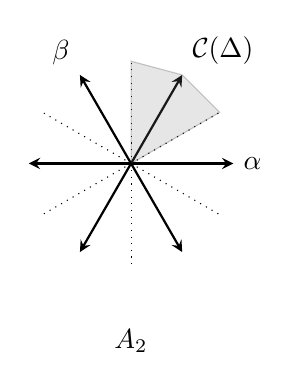
\begin{tikzpicture}[scale=1.5]
        \draw[thick,-stealth](0,0) to (60:{sqrt(3)/2}) node [above right] {$\mc{C}(\D)$};
        \draw[thick,-stealth](0,0) to (240:{sqrt(3)/2});
        \draw[thick,-stealth](0,0) to (180:{sqrt(3)/2});
        \draw[thick,-stealth](0,0) to (360:{sqrt(3)/2}) node [right] {$\a$};
        \draw[thick,-stealth] (0:0) to (120:{sqrt(3)/2}) node [above left] {$\b$};
        \draw[thick,-stealth] (0:0) to (300:{sqrt(3)/2});
        
        \draw[dotted,] (0:0) to (30:{sqrt(3)/2});
        \draw[dotted,] (0:0) to (30:{-sqrt(3)/2});
        \draw[dotted,] (0:0) to (90:{sqrt(3)/2});
        \draw[dotted,] (0:0) to (90:{-sqrt(3)/2});
        \draw[dotted,] (0:0) to (150:{sqrt(3)/2});
        \draw[dotted,] (0:0) to (150:{-sqrt(3)/2});

        \draw[fill=gray,opacity=0.2] (0:0) -- (30:{sqrt(3)/2}) -- (60:{sqrt(3)/2}) -- (90:{sqrt(3)/2}) -- cycle;

        \node at (0,-1.5) {$A_{2}$};
    \end{tikzpicture}
    \end{center}
    
    Given a base $\D$ for $\Phi$, we will require some very useful lemmas about the simple roots $\a \in \D$. Note that the angle between the elements in the base $\D = \{\a,\b\}$ for the type $A_{2}$ root system is obtuse. Our first lemma says that this happens in general:

    \begin{lemma}\label{lem:angles_of_simple_roots_are_obtuse}
        Let $\D$ is a base of $\Phi$ with $\a,\b \in \D$ distinct simple roots. Then $(\a,\b) \le 0$ and $\a-\b$ is not a root.
    \end{lemma}
    \begin{proof}
        Suppose $(\a,\b) > 0$. As $\b \neq -\a$ (for otherwise $\D$ contains $\a$ and $-\a$ and hence is not a basis invalidating property (i) for a base), \cref{lem:sum_or_difference_is_a_root} implies $\a-\b$ is a root. But this contradicts property (ii) for a base. Hence $(\a,\b) \le 0$ and $\a-\b$ is still not a root for otherwise it contradicts property (ii) for a base again.
    \end{proof}

    Our second lemma states that a positive but not simple root is always a sum of a positive root and a simple root:

    \begin{lemma}\label{lem:positive_is_sum_of_simple_base_case}
        If $\a$ is a positive but not simple root, then $\a-\b$ is root for some $\b \in \D$.
    \end{lemma}
    \begin{proof}
        Suppose $(\a,\b) \le 0$ for all $\b \in \D$. Then from \cref{lem:angles_of_simple_roots_are_obtuse} we see that $\D \cup \{\a\}$ form pairwise obtuse angles. By \cref{thm:root_system_base} there exists a $v \in V$ such that $\D = \D(v)$. Then $\D \cup \{\a\}$ all lie on the positive side of $H_{v}$. It follows from \cref{rem:obtuse_independence} that $\D \cup \{\a\}$ is linearly independent which contradictions $\D$ being a basis for $V$ (property (i) for a base). Hence there is some $\b \in \D$ for which $(\a,\b) > 0$. But then \cref{lem:sum_or_difference_is_a_root} implies $\a-\b$ is a root ($\a$ cannot be proportional to $\b$ because $\a$ is not simple).
    \end{proof}

    Note that the root $\a-\b$ in \cref{lem:positive_is_sum_of_simple_base_case} is necessarily positive. Indeed, expressed as a sum of simple roots, $\a-\b$ must have at least one positive coefficient since $\b$ is itself simple and is not proportional to $\a$. By property (ii) of a base it follows that $\a-\b$ is positive. We can actually use \cref{lem:positive_is_sum_of_simple_base_case} to show positive roots can be obtained inductively by adding simple roots:

    \begin{corollary}
        For every $\b \in \Phi^{+}$ there exists, not necessarily distinct, simple roots $\a_{1},\ldots,\a_{k} \in \D$ such that $\b = \a_{1}+\cdots+\a_{k}$ and each partial sum is a root.
    \end{corollary}
    \begin{proof}
        Use \cref{lem:positive_is_sum_of_simple_base_case} and induct on $h(\b)$. 
    \end{proof}
\section{The Weyl Group}
    Throughout this section let $\Phi$ denote a rank $r$. The \textbf{Weyl group} $W$ of $\Phi$ is the subgroup of $\GL(V)$ generated by the reflections $\s_{\a}$ for $\a \in \Phi$. That is,
    \[
        W = \<\s_{\a}:\a \in \Phi\>.
    \]
    If $\D$ is a base for $\Phi$, then the reflection $\s_{\a}$ is said to be a \textbf{simple reflection} if $\a$ is a simple root. Note that property (iii) of a root system implies that $W$ permutes the elements of $\Phi$. Actually, since $\Phi$ is finite this means that $W$ is isomorphic to a subgroup of the symmetric group on $\Phi$. In particular, $W$ is finite. Before proceeding we require a simple lemme about when elements of $\GL(V)$ belong to the Weyl group:

    \begin{lemma}\label{lem:when_linear_transform_is_a_Weyl_group_element}
        Let $\Phi$ be a root system with Weyl group $W$. If $\s \in \GL(V)$ leaves $\Phi$ invariant, fixes pointwise a hyperplane $H$ of $V$, and sends some $\a \in \Phi$ to its negative, then $\s = \s_{\a}$ and $H = H_{\a}$. 
    \end{lemma}
    \begin{proof}
        Let $\tau = \s\s_{\a} = \s\s_{\a}^{-1}$ (the second identity holds because $\s_{\a}$ is a reflection). Then $\tau$ leaves $\Phi$ invariant and $\tau(\a) = \a$. In particular, $\tau$ acts as the identity on the subspace $\R\a$. Actually, the induced action of $\tau$ acts as the identity on the quotient space $V/\R\a$. To see this, since $\s$ fixes $H$ pointwise and sends $\a$ to its negative, we conclude $\a \notin H$. But as $H$ has codimension $1$, it follows that $V = H \op \R\a$. On the other hand, $V = H_{\a} \op \R\a$. These two decompositions together imply $H = H_{\a}$ and so $V/\R\a \cong H_{\a} = H$. It follows that the induced action of $\tau$ on $V/\R\a$ acts as the identity. So all of the eigenvalues of $\tau$ are $1$. But then the minimal polynomial for $\tau$ divides $(T-1)^{r}$. Now choose some $\b \in \Phi$ and let $n > |\Phi|$. Then the roots $\tau(\b),\ldots,\tau^{n}(\b)$ cannot all be distinct so some power of $\tau$ fixes $\b$. Since $|\Phi|$ is finite, choose $n$ large enough so that $\tau^{n}$ fixes $\Phi$ pointwise. Since $\Phi$ spans $V$ (property (i) of a root system), $\tau^{n} = 1$. But then the minimal polynomial for $\tau$ divides $T^{n}-1$. Hence the minimal polynomial divides the $((T-1)^{r},T^{n}-1) = T-1$. But then $\tau = 1$ and using $\tau = \s\s_{\a}^{-1}$ we find that $\s = \s_{\a}$.
    \end{proof}

    We can now show how certain elements of $\GL(V)$ act by conjugation on elements of the Weyl group:

    \begin{lemma}\label{lem:Weyl_group_conjugation}
        Let $\Phi$ be a root system with Weyl group $W$. If $\s \in \GL(V)$ leaves $\Phi$ invariant then $\s\s_{\a}\s^{-1} = \s_{\s(\a)}$ for all $\a \in \Phi$. Moreover, $\<\b,\a\> = \<\s(\b),\s(\a)\>$ for all $\a,\b \in \Phi$.
    \end{lemma}
    \begin{proof}
        Let $\b \in \Phi$ and observe $\s\s_{\a}\s^{-1}(\s(\b)) = \s(\s_{\a}(\b))$. But as $\s_{\a}(\b) \in \Phi$ and by assumption $\s$ leaves $\Phi$ invariant, we conclude $\s(\s_{\a}(\b)) \in \Phi$. Now as $\b$ run over $\Phi$, $\s(\b)$ runs over $\Phi$ and we see that $\s\s_{\a}\s^{-1}$ leves $\Phi$ invariant. Moreover, linearity of $\s$ implies
        \[
            \s\s_{\a}\s^{-1}(\s(\b)) = \s(\s_{\a}(\b)) = \s(\b-\<\b,\a\>\a) = \s(\b)-\<\b,\a\>\s(\a).
        \]
        So taking $\b = \a$ we see that $\s\s_{\a}\s^{-1}(\s(\a)) = -\s(\a)$ because $\<\a,\a\> = 2$. An analgous computation shows $\s\s_{\a}\s^{-1}$ fixes $\s(H_{\a})$ pointwise. So altogether, $\s\s_{\a}\s^{-1}$ leves $\Phi$ invariant, fixes $\s(H_{\a})$ pointwise, and sends $\s(\a) \in \Phi$ to its negative. By \cref{lem:when_linear_transform_is_a_Weyl_group_element}, $\s\s_{\a}\s^{-1} = \s_{\s(\a)}$. But now
        \[
            \s_{\s(\a)}(\s(\b)) = \s(\b)-\<\s(\b),\s(\a)\>\s(\a),
        \]
        and since $\s\s_{\a}\s^{-1} = \s_{\s(\a)}$, we conclude that $\<\b,\a\> = \<\s(\b),\s(\a)\>$.
    \end{proof}

    More generally, we say two root systems $\Phi_{1}$ and $\Phi_{2}$ corresponding to Euclidean vector spaces $V$ are isomorphic if there is an invertible linear transformation $\phi:V \to V$ such that
    \[
        \phi(\Phi_{1}) = \Phi_{2} \quad \text{and} \quad \<\b,\a\> = \<\phi(\b),\phi(\a)\>,
    \]
    for all $\a,\b \in \Phi_{1}$. It follow from \cref{lem:Weyl_group_conjugation} that $\phi$ induces a natural isomorphism on their Weyl groups $W_{1}$ and $W_{2}$ given by $\s \mapsto \phi\s\phi^{-1}$ for $\s \in W_{1}$. More generally, from \cref{lem:Weyl_group_conjugation} we see that an automorphism of $\Phi$ is just an automorphism of $V$ that leaves $\Phi$ invariant. In particular, $W$ is a subgroup of $\Aut(\Phi)$.

    We are now ready for some lemmas about simple reflections. After proving all of these lemmas, we will use them to essentially characterise the Weyl group $W$ with respect to a base $\D$. First up, the simple reflections permute all positive roots except one:

    \begin{lemma}\label{lem:simple_reflections_permute_positive_roots}
        Any simple reflection $\s_{\a}$ permutes the positive roots other than $\a$.
    \end{lemma}
    \begin{proof}
        Let $\b \in \Phi^{+}-\{\a\}$. Recall that $\s_{\a}$ adds a multiple of $\a$ to $\b$ given by
        \[
            \s_{\a}(\b) = \b-\<\b,\a\>\a.
        \]
        As $\b$ is not proportional to $\a$ (the only proportional root is $-\a$ and $\b$ is positive), when $\b$ is expressed as a sum of simple roots it must have a positive coefficient corresponding to some simple root other than $\a$. But then $\s_{\a}(\b)$ must be positive because $\s_{\a}$ only changes the coefficient of $\a$. Moreover, $\s_{\a}(\b) \neq \a$ because $\b \neq -\a$. As $\b$ was an arbitrary positive root and $\s_{\a}$ is a bijection, $\s_{\a}$ must permute the set $\Phi^{+}-\{\a\}$.
    \end{proof}

    As an application of \cref{lem:simple_reflections_permute_positive_roots}, define the \textbf{Weyl vector} $\rho$ to be the half-sum of all the positive roots. In other words, $\rho$ is given by
    \[
        \rho = \frac{1}{2}\sum_{\b > 0}\b.
    \]
    Note that the Weyl vector is not a root because it is not an integral sum of roots. Nevertheless, the action of simple reflections on the Weyl vector is easily expressed:

    \begin{corollary}\label{cor:simple_reflection_on_half_sum_element}
        If $\s_{\a}$ is a simple reflection, then $\s_{\a}(\rho) = \rho-\a$.
    \end{corollary}
    \begin{proof}
        By the linearity of $\s_{\a}$ and \cref{lem:simple_reflections_permute_positive_roots}, we have
        \[
            \s_{\a}(\rho) = \s_{\a}\left(\frac{1}{2}\sum_{\b > 0}\b\right) = \frac{1}{2}\sum_{\substack{\b > 0 \\ \b \neq \a}}\b+\frac{1}{2}\s_{\a}(\a) = \frac{1}{2}\sum_{\substack{\b > 0 \\ \b \neq \a}}\b-\frac{1}{2}\a = \rho-\a.
        \]
    \end{proof}

    Our last lemma tells us when we can remove a simple reflection from a product of simple reflections:

    \begin{lemma}\label{lem:removing_simple_reflection}
        Let $\a_{1},\ldots,\a_{t} \in \D$ be, not necessarily distinct, simple roots. If $\s_{\a_{1}} \cdots \s_{\a_{t-1}}(\a_{t})$ is a negative root, then there exists some $s$ with $1 \le s < t$ such that
        \[
            \s_{\a_{1}} \cdots \s_{\a_{t}} = \s_{\a_{1}} \cdots \s_{\a_{s-1}}\s_{\a_{s+1}} \cdots \s_{\a_{t}}.
        \]
    \end{lemma}
    \begin{proof}
        Set $\b_{i} = \s_{\a_{i+1}} \cdots \s_{\a_{t-1}}(\a_{t})$ for $0 \le i \le t-2$ and $\b_{t-1} = \a_{t}$. Then by assumption $\b_{0} < 0$. But as $\b_{t-1} > 0$, there exists a minimal $s$ with $1 \le s < t$ such that $\b_{s} > 0$. Since $s$ is minimal, $\b_{s-1} = \s_{\a_{s}}(\b_{s}) < 0$. By \cref{lem:simple_reflections_permute_positive_roots}, we find that $\b_{s} = \a_{s}$ and so we know $\s_{\b_{s}} = \s_{\a_{s}}$. But from \cref{lem:Weyl_group_conjugation} we also know
        \[
            \s_{\b_{s}} = (\s_{\a_{s+1}} \cdots \s_{\a_{t-1}})\s_{\a_{t}}(\s_{\a_{s+1}} \cdots \s_{\a_{t-1}})^{-1} = (\s_{\a_{s+1}} \cdots \s_{\a_{t-1}})\s_{\a_{t}}(\s_{\a_{t-1}} \cdots \s_{\a_{s+1}}).
        \]
        Combining these two expressions for $\s_{\b_{s}}$ yields
        \[
            \s_{\a_{s}} = (\s_{\a_{s+1}} \cdots \s_{\a_{t-1}})\s_{\a_{t}}(\s_{\a_{t-1}} \cdots \s_{\a_{s+1}}),
        \]
        and so
        \[
            \s_{\a_{1}} \cdots \s_{\a_{t}} = \s_{\a_{1}} \cdots \s_{\a_{s-1}}\s_{\a_{s+1}} \cdots \s_{\a_{t}}.
        \]
    \end{proof}

    We also have the nice corollary that tells us when we do not have a minimal expression for an element of $W$ in terms of simple reflections:

    \begin{corollary}\label{cor:reflection_of_first_root_is_negative}
        Let $\s \in W$ be a non-identity element and let $\a_{1},\ldots,\a_{t} \in \D$ be, not necessarily distinct, simple roots chosen such that $\s = \s_{\a_{1}} \cdots \s_{\a_{t}}$ with $t$ minimal. Then $\s(\a_{t}) < 0$. 
    \end{corollary}
    \begin{proof}
        Note that as $\s$ is not the identity, $t \ge 1$. If $t = 1$ then $\s = \s_{\a_{t}}$ and the result is trivial. So suppose $t > 2$. Observe, by linearity, that
        \[
            \s(\a_{t}) = \s_{\a_{1}} \cdots \s_{\a_{t-1}}(-\a) = -\s_{\a_{1}} \cdots \s_{\a_{t-1}}(\a).
        \]
        So if $\s(\a_{t}) > 0$ then $\s_{\a_{1}} \cdots \s_{\a_{t-1}}(\a) < 0$ and \cref{lem:removing_simple_reflection} implies that one of the simple reflections $\s_{\a_{s}}$ with $1 \le s < t$ in the expression for $\s$ can be removed. But this contradicts the minimality of $t$. Hence $\s(\a_{t}) < 0$.
    \end{proof}

    Using all of these lemmas we will prove that $W$ permutes the bases of $\Phi$ (equivalently the Weyl chambers) simply transitively and that $W$ is generated by the simple reflections:

    \begin{theorem}\label{thm:Weyl_action_simply_transitively}
        Let $\Phi$ be a root system with base $\D$ and Weyl group $W$. Then the following are true:
        \begin{enumerate}[label=(\roman*)]
            \item If $v \in V$ is regular, then there exists $\s \in W$ such that $(\s(v),\a) > 0$ for all $a \in \D$. In particular, for any chamber $\mc{C}$ there is a $\s \in W$ such that $\s(\mc{C}) = \mc{C}(\D)$.
            \item If $\D'$ is another base of $\Phi$, then $\s(\D') = \D$ for some $\s \in W$.
            \item If $\a$ is any root, then there exists $\s \in W$ such that $\s(\a) \in \D$.
            \item $W$ is generated by the simple reflections $\s_{\a}$ with $\a \in \D$.
            \item If $\s(\D) = \D$ for some $\s \in W$, then $\s = 1$.
            \item If $\s(\mc{C}) = \mc{C}$ for some $\s \in W$, then $\s = 1$.
        \end{enumerate}
    \end{theorem}
    \begin{proof}
        We will prove each statment individually. Let $W'$ be the subgroup of $W$ generated by the simple reflections $\s_{\a}$ with $\a \in \D$. We will first prove statements (i)-(iii) with $W'$ in place of $W$. Call these statements (i')-(iii'). Then we will prove statement (iv), that is $W' = W$, which will imply (i)-(iii). Lastly we will prove statements (v) and (vi).
        \begin{enumerate}[label=(\roman*')]
            \item Choose $\s \in W'$ such that $(\s(v),\rho)$ is as large as possible (such a $\s$ exists because $W'$ is finite). If $\a$ is a simple root, then $\s_{\a}\s \in W'$ and so \cref{cor:simple_reflection_on_half_sum_element} together with the fact that $\s_{\a}$ is an isometry imply
            \[
                (\s(v),\rho) \ge (\s_{\a}\s(v),\rho) = (\s(v)\s_{\a}(\rho)) = (\s(v),\rho-\a) = (\s(v),\rho)-(\s(v),\a).
            \]
            It follows that $(\s(v),\a) \ge 0$ for all $\a \in \D$. By \cref{lem:Weyl_group_conjugation} again, $(\s(v),\a) = (v,\s^{-1}(\a))$. Since $v$ is regular, $(\s(v),\a) = (v,\s(\a)) \neq 0$ for otherwise $v$ is orthogonal to $\s^{-1}(\a) \in \Phi$ which means $v \in H_{\s^{-1}(\a)}$. Therefore we actually have the strict inequality $(\s(v),\a) > 0$ for all $\a \in \D$. The second statement follows immeditely since $v$ was arbitrary.
            \item Since any $\s \in W'$ is a linear isomorphism, it sends a basis to a basis. Therefore $\s(\D')$ satsifies property (i) for a base. Actually, since $\s$ is linear property (ii) for a base is also satisfied. Hence $\s(\D')$ is some base. As $W$ acts by isometries, we have
            \begin{align*}
                \s(\mc{C}(\D')) &= \{\s(v) \in V:(v,\a) > 0 \text{ for all } \a \in \D'\} \\
                &= \{\s(v) \in V:(\s(v),\s(\a)) > 0 \text{ for all } \a \in \D'\} \\
                &= \{v \in V:(v,\s(\a)) > 0 \text{ for all } \a \in \D'\} \\
                &= \{v \in V:(v,\a) > 0 \text{ for all } \a \in \s(\D')\} \\
                &= \mc{C}(\s(\D')),
            \end{align*}
            where the last line follows because $\s(\D')$ is a base. On the other hand, let $v \in \mc{C}(\D')$ so that $\mc{C}(\D') = \mc{C}(v)$. Then by statement (i'), there exists $\s \in W'$ such that $\s(\mc{C}(\D')) = \s(\mc{C}(v)) = \mc{C}(\D)$. Equating these two expressions for $\s(\mc{C}(\D'))$ we find that $\mc{C}(\s(\D')) = \mc{C}(\D)$. Since the Weyl chambers are in bijection with bases, this implies $\s(\D') = \D$.
            \item In light of statement (ii'), it suffices to show that every root $\a \in \Phi$ belongs to some base. To see this, note that the hyperplanes $H_{\b}$ with $\b \neq \pm\a$ are distinct from $H_{\a}$ (because the only root proportional to $\a$ is itself and $-\a$). Since there are finitely many such hyperplanes, we can choose some $v \in H_{\a}$ such that $v \notin H_{\b}$ for all $\b$. Now let $\e > 0$. Then by taking $v' \in V$ close enough to $v$ we guarantee $(v',\a) = \e > 0$ and $|(v',\b)| > \e$ for all $\b$. But then $\a \in \D(v')$.
        \end{enumerate}
       Having verified statements (i')-(iii'), we now prove statement (iv):
        \begin{enumerate}[label=(\roman*)]
            \setcounter{enumi}{3}
            \item It suffices to prove $W' = W$. As $W'$ is a subgroup of $W$, it further suffices to show that $\s_{\a} \in W'$ for every $\a \in \Phi$. By statement (iii'), find $\s \in W'$ such that $\b = \s(\a) \in \D$. But then \cref{lem:Weyl_group_conjugation} implies
            \[
                \s_{\b} = \s_{\s(a)} = \s\s_{\a}\s^{-1}.
            \]
            As $\b$ is a simple root and $\s \in W'$, we conclude $\s_{\a} = \s^{-1}\s_{\b}\s \in W'$.
        \end{enumerate}
        Since we have vertified statement (iv), it follows that (i)-(iii) hold because (i')-(iii') do. At last we prove statements (v) and (vi):
        \begin{enumerate}[label=(\roman*)]
            \setcounter{enumi}{4}
            \item We will prove this by contradiction. suppose $\s(\D) = \D$ but that $\s \neq 1$. By (iv), write $\s$ as a minimal product of simple reflections. But then $\s(\a_{t}) \in \D$ is a positive root which contradicts \cref{cor:reflection_of_first_root_is_negative}. Hence $\s = 1$.
            \item Arguing as in proof of statement (ii'), $\s(\mc{C}) = \mc{C}$ implies $\s(\D(\mc{C})) = \D(\mc{C})$. By (v) it follows that $\s = 1$.
        \end{enumerate}
    \end{proof}

    Note that statements (i) and (vi) of \cref{thm:Weyl_action_simply_transitively} together say that $W$ acts transitively on the Weyl chambers. Similarly, statements (ii) and (v) together say that $W$ acts simply transitively on bases. Since there is a natural bijection between Weyl chambers and bases it follows immeditely that the action of $W$ preserves this correspondence. Also, from statement (iv) we know that every element of $W$ can be written as a product of simple refections for a fixed base $\D$. Accordingly, we define the \textbf{length} $\ell(\s)$ of any non-identity $\s \in W$, relative to $\D$, to be the smallest positive integer such that
    \[
        \s = \s_{\a_{1}} \cdots \s_{\a_{\ell(\s)}},
    \]
    with $\a_{1},\ldots,\a_{\ell(\s)} \in \D$ (not necessarily distinct). We call this expression the \textbf{reduced form} of $\s$ relatively to $\D$. By definition we set $\ell(1) = 0$. We can also characterize the length of roots in another way. For any $\s \in W$ let $n(\s)$ be the number of positive roots $\a \in \Phi^{+}$ such that $\s(\a) \in \Phi^{-}$. Then we have the following proposition:

    \begin{proposition}
        For all $\s \in W$, $\ell(\s) = n(\s)$.
    \end{proposition}
    \begin{proof}
        We will prove this by strong induction on $\ell(\s)$. The case $\ell(\s)$ is clear since then $\s = 1$. Now assume the statement is true for all $\tau \in W$ with $\ell(\tau) < \ell(\s)$. Now suppose $\s = \s_{\a_{1}} \cdots \s_{\a_{\ell(\s)}}$ is the reduced form for $\s$ (where $\a_{1},\ldots,\a_{\ell(\s)} \in \D$). Now for ease of notation set $\a = \a_{\ell(\s)}$. Then \cref{cor:reflection_of_first_root_is_negative} implies $\s(\a) < 0$ and so $\s\s_{\a}(\a) > 0$. But then from \cref{lem:simple_reflections_permute_positive_roots} we see that $n(\s\s_{\a}) = n(\s)-1$. On the other hand, $\ell(\s\s_{\a}) = \ell(\s)-1$. But $\ell(\s)-1 < \ell(\s)$ so by induction our previous two equalities imply $n(\s)-1 = \ell(\s)-1$. Therefore $\ell(\s) = n(\s)$ and the induction is complete.
    \end{proof}

    Returning to the Weyl group, we can also compute the order of the product of two simple reflections:

    \begin{proposition}\label{prop:order_of_product_of_simple_reflections}
        Let $\Phi$ be a root system with base $\D$ and Weyl group $W$. For any two distinct $\a,\b \in \D$, the order of $\s_{\a}\s_{\b}$ is $2$, $3$, $4$, or $6$, depending on if $\<\a,\b\>\<\b,\a\>$ is $0$, $1$, $2$, or $3$ respectively. 
    \end{proposition}
    \begin{proof}
        If $\t$ is the angle between $\a$ and $\b$, then $\s_{\a}\s_{\b}$ is a rotation through angle $2\t$. The statement now follows from \cref{tab:root_angles}.
    \end{proof}

    Lastly, we prove that the closure of the fundamental Weyl chamber $\mc{C}(\D)$ relative to the base $\D$ is a fundamental domain for the action of $W$ on $V$:

    \begin{proposition}\label{prop:fundamental_domain}
        For any base $\D$, $\overline{\mc{C}(\D)}$ is a fundamental domain for the action of $W$ on $V$.
    \end{proposition}
    \begin{proof}
        We first show that every $v \in V$ is $W$-equivalent to some point of $\overline{\mc{C}(\D)}$. This is immediate since $W$ acts simply transitively on the Weyl chambers by \cref{thm:Weyl_action_simply_transitively} and
        \[
            V = \bigcup_{\mc{C}}\overline{\mc{C}}.
        \]
        Now suppose $v,w \in \overline{\mc{C}(\D)}$ and there exists some non-identity $\s \in W$ such that $\s v = w$. We will show $v$ and $w$ lie on the boundary of $\overline{\mc{C}(\D)}$. As the reflections $\s \in W$ are homeomorphisms, they are also open maps. So $v$ and $w$ are either both interior points or both boundary boints. Suppose, to the contrary, that $v,w \in \mc{C}(\D)$. Then as $\s$ is a homeomorphism and $\s(v) = w$, $\s(\mc{C}(\D)) = \mc{C}(\D)$. But then $\s = 1$ because $W$ acts simily transitively on the Weyl chambers. But this contradicts $\s$ being a non-identity element. Hence $v$ and $w$ are on the bounary of $\mc{C}(\D)$. Lastly, $\overline{\mc{C}(\D)}$ is path-connected because $\mc{C}(\D)$ is open and $V$ is complete. Altogether, we have shown that $\mc{C}(\D)$ is a fundamental domain for the action of $W$ on $V$.
    \end{proof}
\section{Irreducible Root Systems}
    It is possible to classify root systems completely. In order to do this, we need the notion of when a root system cannot be decomposed into two smaller root systems. We say that a root system $\Phi$ is \textbf{reducible} if there exists a nontrivial partition $\Phi = \Phi_{1} \cup \Phi_{2}$ such that the roots in $\Phi_{1}$ and $\Phi_{2}$ are pairwise orthogonal. This last condition means $(\Phi_{1},\Phi_{2}) = 0$. Otherwise, we say $\Phi$ is \textbf{irreducible}. Similarly, given a base $\D$ we say that $\D$ is \textbf{reducible} if there exists a nontrivial partition $\D = \D_{1} \cup \D_{2}$ such that the simple roots in $\D_{1}$ and $\D_{2}$ are pairwise orthogonal. Again, this last condition means $(\D_{1},\D_{2}) = 0$. Otherwise, we say $\D$ is \textbf{irreducible}. It turns out that irreducibility of $\Phi$ is equivalent to that of $\D$:
    
    \begin{proposition}\label{prop:irreducibility_equivalence}
        Let $\Phi$ be a root system with base $\D$. Then $\Phi$ is irreducible if and only if $\D$ is.
    \end{proposition}
    \begin{proof}
        We will show the equivalent statement that $\Phi$ is reducible if and only if $\D$ is. So suppose $\Phi = \Phi_{1} \cup \Phi_{2}$ is reducible and note that $(\Phi_{1},\Phi_{2}) = 0$. Unless $\D$ is contained in $\Phi_{1}$ or $\Phi_{2}$, this nontrivial parition of $\Phi$ induces a nontrivial parition $\D = \D_{1} \cup \D_{2}$ with $(\D_{1},\D_{2}) = 0$ as desired. So without loss of generality suppose $\D \subset \Phi_{1}$. Then $(\D,\Phi_{2}) = 0$ and this impies $(V,\Phi_{2}) = 0$ because $\D$ spans $V$. But then $\Phi_{2} = \{\textbf{0}\}$ so that the parition is $\Phi = \Phi_{1} \cup \Phi_{2}$ is trivial which contradicts $\Phi$ being reducible. This proves the ``if'' implication. For the ``only if'', we will prove by contradiction. So suppose $\Phi$ is irreducible but that $\D = \D_{1} \cup \D_{2}$ is reducible. Note that $(\D_{1},\D_{2}) = 0$. By \cref{thm:Weyl_action_simply_transitively} (statement (iii)), every root is the $W$-image of some simple root in $\D$. Therefore the nontrivial decomposition $\D = \D_{1} \cup \D_{2}$ induces a nontrivial decomposition $\Phi = \Phi_{1} \cup \Phi_{2}$ where $\Phi_{i} = W(\D_{i})$ for $1 \le i \le 2$. Now observe that if $(\a,\b) = 0$ then $\s_{\a}(\b) = \b$. Since \cref{thm:Weyl_action_simply_transitively} (statement (iv)) states that $W$ is generated by simple reflections, our previous observation implies that each root in $\Phi_{i}$ is a linear combination of those simple roots in $\D_{i}$ obtained by applying the corresponding $\s \in W$ written as a product of simple reflections. In particular $\Phi_{i}$ is contained in the span of $\D_{i}$. Therefore $(\D_{1},\D_{2}) = 0$ implies $(\Phi_{1},\Phi_{2}) = 0$. But then $\Phi$ is reducible which is a contradiction.
    \end{proof}

    \cref{prop:irreducibility_equivalence} says that to check irreducibility for a root system it suffices to check irreducibility on any base.

    As for some examples, it is clear that the root system of type $A_{2}$ is irreducible. Indeed, no root is orthogonal to all other roots. As for a non-example, the root system of type $A_{1} \x A_{1}$ is the simplest such (here the dotted lines have been supressed because they are covered by roots):

    \begin{center}
    \begin{tikzpicture}[scale=1.5]
        \draw[thick,-stealth](0,0) to (180:{sqrt(3)/2});
        \draw[thick,-stealth](0,0) to (360:{sqrt(3)/2}) node [right] {$\a$};
        \draw[thick,-stealth](0,0) to (90:{sqrt(3)/2}) node [above] {$\b$};
        \draw[thick,-stealth](0,0) to (270:{sqrt(3)/2});

        \node at (0,-1.5) {$A_{1} \x A_{1}$};
    \end{tikzpicture}
    \end{center}
    
    We will now prove some interesting properties of irreducible root systems. The first is that irreducible root systems have a highest root with respect to the partial ordering $<$ induced by height:
    
    \begin{proposition}\label{prop:highest_root}
        Let $\Phi$ be a root system with base $\D$. If $\Phi$ is irreducible then there is a unique maximal root $\b$ relative to the base $\D$ and the partial ordering $<$. Writing $\b = \sum_{\a \in \D}k_{\a}\a$, we have $k_{\a} > 0$ for all $\a$. Moreover, $(\a,\b) \ge 0$ for all $\a \in \D$ and at least one of these inequalities is strict.
    \end{proposition}
    \begin{proof}
        Let $\b = \sum_{\a \in \D}k_{\a}\a$ be maximal with respect to the partial ordering $<$ (such an element exists because $\Phi$ is finite). Clearly $\b > 0$. Now set
        \[
            \D_{1} = \{\a \in \D:k_{\a} > 0\} \quad \text{and} \quad \D_{2} = \{\a \in \D:k_{\a} = 0\}.
        \]
        Then $\D = \D_{1} \cup \D_{2}$ is a partition of $\D$. As $\Phi$ is irreducible, \cref{prop:irreducibility_equivalence} implies that one of $\D_{1}$ or $\D_{2}$ is empty. We will show $\D_{2}$ is empty by contradiction. So suppose $\a \in \D_{2}$. Then $(\a,\b) \le 0$ by \cref{lem:angles_of_simple_roots_are_obtuse}. But $\Phi$ is irreducible so there must be some $\a' \in \D_{1}$ that is not orthogonal to $\a$. By \cref{lem:angles_of_simple_roots_are_obtuse} again, $(\a,\a') < 0$ and therefore $(\a,\b) < 0$. But then \cref{lem:sum_or_difference_is_a_root} implies $\a+\b$ is a root which contradicts the maximality of $\b$. Therefore $\D_{2}$ is empty and thus all $k_{\a} > 0$. Moreover, if $(\a,\b) < 0$ with $\a \in \D$, then arguing just as before, \cref{lem:sum_or_difference_is_a_root} implies $\a+\b$ is a root contradicting the maximality of $\b$. So altogether we have shown $k_{\a} > 0$ and $(\a,\b) \ge 0$ for all $\a \in \D$. In particular, as $\D$ spans $V$ and $\b \neq 0$ there must be some $\a \in \D$ where $(\a,\b) \ge 0$ must be strict. The last thing we have to show is that $\b$ is unique. Suppose $\b'$ is another such maximal root. Then the preceding argument applies to $\b'$ as well and it follows that $(\b,\b') > 0$. By \cref{lem:sum_or_difference_is_a_root}, $\b-\b'$ is a root unless $\b = \b'$. But if $\b-\b'$ is a root then it is either positive or negative so that $\b < \b'$ or $\b' < \b$ both of which contradict the maximality of $\b$ or $\b'$. Hence $\b = \b'$ proving that $\b$ is unique.
    \end{proof}

    We call the unique root $\b$ established in \cref{prop:highest_root} the \textbf{highest root} of $\Phi$ relative to $\D$. Note that as $(\a,\b) \ge 0$ for all $\a \in \D$, $\b \in \overline{C(\D)}$.

    For the type $A_{2}$ root system with base $\D = \{\a,\b\}$, the highest root is $\a+\b$:
    
    \begin{center}
    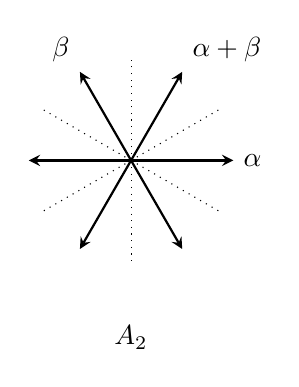
\begin{tikzpicture}[scale=1.5]
        \draw[thick,-stealth](0,0) to (60:{sqrt(3)/2}) node [above right] {$\a+\b$};
        \draw[thick,-stealth](0,0) to (240:{sqrt(3)/2});
        \draw[thick,-stealth](0,0) to (180:{sqrt(3)/2});
        \draw[thick,-stealth](0,0) to (360:{sqrt(3)/2}) node [right] {$\a$};
        \draw[thick,-stealth] (0:0) to (120:{sqrt(3)/2}) node [above left] {$\b$};
        \draw[thick,-stealth] (0:0) to (300:{sqrt(3)/2});
        
        \draw[dotted,] (0:0) to (30:{sqrt(3)/2});
        \draw[dotted,] (0:0) to (30:{-sqrt(3)/2});
        \draw[dotted,] (0:0) to (90:{sqrt(3)/2});
        \draw[dotted,] (0:0) to (90:{-sqrt(3)/2});
        \draw[dotted,] (0:0) to (150:{sqrt(3)/2});
        \draw[dotted,] (0:0) to (150:{-sqrt(3)/2});

        \node at (0,-1.5) {$A_{2}$};
    \end{tikzpicture}
    \end{center}

    The second property is that if the root system $\Phi$ is irreducible, then the Weyl group $W$ acts irreducibly on $V$. That is, there are no nontrivial $W$-invariant subspaces:

    \begin{proposition}\label{prop:Weyl_group_acts_irreducibly}
        If $\Phi$ is irreducible, then $W$ acts irreducibly on $V$.
    \end{proposition}
    \begin{proof}
        Let $U$ be a $W$-invariant supace of $V$. We need to show $U$ is either the zero subspace or all of $V$. Letting $U^{\perp}$ be the orthogonal complement to $U$ in $V$, we have $V = U \op U^{\perp}$. Since $W$ acts by isometries it follows that $U^{\perp}$ is also a $W$-invariant subspace. Now for $\a \in \Phi$, $\s_{\a}$ leaves $H_{\a}$ invariant so either $H_{\a} \subseteq U$ or $H_{\a} \subseteq U^{\perp}$. As $\a$ is orthogonal to $H_{\a}$, in the first case $\a \in U^{\perp}$ and in the second case $\a \in U$. Since $\a$ was an arbitrary root, any root in $\Phi$ either lies in $U$ or $U^{\perp}$. This induces a parition $\Phi = \Phi_{1} \cup \Phi_{2}$ with $\Phi_{1} \subset U$, $\Phi_{2} \subset U^{\perp}$ and $(\Phi_{1},\Phi_{2}) = 0$. Since $\Phi$ is irreducible, this parition must be trivial so that either $\Phi_{1}$ or $\Phi_{2}$ is empty. But as $\Phi_{1}$ spans $U$ and $\Phi_{2}$ spans $U^{\perp}$ (otherwise $\Phi$ does not span $V$ contradicting property (i) of a root system), we must have that either $U$ or $U^{\perp}$ is the zero subspace. Hence $U$ is either the zero subspace or all of $V$.
    \end{proof}

    Our third property is that there are at most two choices for the lengths of the roots in an irreducible root system. Actually, we will show that $W$ acts transitively on the set of roots with the same length:

    \begin{proposition}\label{prop:two_root_lengths}
        If $\Phi$ is irreducible, then there are most two lengths for any root in $\Phi$. Moreover, $W$ acts transitively on the subset of roots with the same length.
    \end{proposition}
    \begin{proof}
        Suppose $\a,\b,\g \in \Phi$ are roots of all different lengths with $|\a| < |\b| < |\g|$. By \cref{prop:Weyl_group_acts_irreducibly} the set $\{\s(\a):\a \in \Phi\}$ spans $V$. Therefore there are elements $\s,\tau \in W$ such that $\a' = \s(\a)$ is not orthogonal to $\b$ and $\a'' = \tau(\a)$ is not orthogonal to $\g$. Moreover, $W$ acts by isometries so that $|\a''| = |\a'| = |\a|$. So from \cref{tab:root_angles}, we see that the ratios $\frac{|\b|^{2}}{|\a|^{2}}$ and $\frac{|\g|^{2}}{|\a|^{2}}$ exist and in particular $\frac{|\b|^{2}}{|\a|^{2}} = 2$ while $\frac{|\g|^{2}}{|\a|^{2}} = 3$. Using \cref{prop:Weyl_group_acts_irreducibly} again but for $\b$, we can find an $\eta \in W$ such that $\beta' = \eta(\beta)$ is not orthogonal to $\g$ and again $|\b'| = |\b|$. But then $\frac{|\g|}{|\b|}$ is defined and from \cref{tab:root_angles} we have $\frac{|\g|^{2}}{|\b|^{2}} \in \left\{2,3\right\}$. On the other hand, our work above implies
        \[
            \frac{|\g|^{2}}{|\b|^{2}} = \frac{|\g|^{2}}{|\a|^{2}}\frac{|\a|^{2}}{|\b|^{2}} = \frac{3}{2},
        \]
        which contradicts \cref{tab:root_angles}. Therefore there are at most two root lengths. We now show that $W$ acts transitively on the subset of roots with the same length. So suppose $\a,\b \in \Phi$ have the same length. Appealing to \cref{prop:Weyl_group_acts_irreducibly} again (replacing $\a$ with $\s(\a)$ for some $\s \in W$ if necessary), we may assume $\a$ and $\b$ are not orthogonal. If $\b = \pm \a$ then the argument is trivial so additionally suppose $\b \neq \pm\a$. As $\frac{|\b|^{2}}{|\a|^{2}} = 1$, we determine from \cref{tab:root_angles} that $\<\b,\a\> = \<\a,\b\> = \pm 1$. Replacing $\b$ by $-\b$ if necessary (we can do this becase $-\b = \s_{\b}(\b)$), we may assume $\<\a,\b\> = 1$. Then
        \[
            \s_{\a}\s_{\b}\s_{\a}(\b) = \s_{\a}\s_{\b}(\b-\a) = \s_{\a}\s_{\b}(\b)-\s_{\a}\s_{\b}(\a) = -\s_{\a}(\b)-\s_{\a}(\a-\b) = -\s_{\a}(\a) = \a.
        \]
        In other words, if $\s = \s_{\a}\s_{\b}\s_{\a}$, then $\s(\b) = \a$. Since $\a$ and $\b$ were arbitrary, it follows that $W$ acts transitively on the subset of roots of the same length.
    \end{proof}

    In accordance with \cref{prop:two_root_lengths}, if an irreducible root system $\Phi$ has two distinct lengths of roots, we call any corresponding root a \textbf{long root} or \textbf{short root} respectively. If every root in an irreducible root system $\Phi$ has the same length, we take the roots to be long by convention. Moreover, in this case we say that $\Phi$ is \textbf{simply laced}.
    
    An example of a non-simply laced root system is that of type $B_{2}$ (here the dotted lines have also been supressed since they are covered by roots):

    \begin{center}
    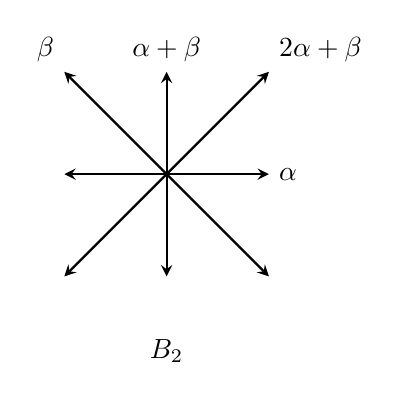
\begin{tikzpicture}[scale=1.5]
        \draw[thick,-stealth](0,0) to (180:{sqrt(3)/2});
        \draw[thick,-stealth](0,0) to (360:{sqrt(3)/2}) node [right] {$\a$};
        \draw[thick,-stealth](0,0) to (90:{sqrt(3)/2}) node [above] {$\a+\b$};
        \draw[thick,-stealth](0,0) to (270:{sqrt(3)/2});
        \draw[thick,-stealth](0,0) to (45:{sqrt(3)/(2*cos(45))}) node [above right] {$2\a+\b$};
        \draw[thick,-stealth](0,0) to (135:{sqrt(3)/(2*cos(45))}) node [above left] {$\b$};
        \draw[thick,-stealth](0,0) to (225:{sqrt(3)/(2*cos(45))});
        \draw[thick,-stealth](0,0) to (315:{sqrt(3)/(2*cos(45))});


        \draw[dotted,] (0:0) to (90:{sqrt(3)/2});
        \draw[dotted,] (0:0) to (90:{-sqrt(3)/2});
        \draw[dotted,] (0:0) to (0:{sqrt(3)/2});
        \draw[dotted,] (0:0) to (0:{-sqrt(3)/2});

        \node at (0,-1.5) {$B_{2}$};
    \end{tikzpicture}
    \end{center}

    For the root system of type $B_{2}$, $\D = \{\a,\b\}$ is a base, $\b$ is the long root while $\a$ is the short root and $2\a+\b$ is the highest root relative to the base $\D$.
    
    If $\D$ is a base of $\Phi$, then the highest root $\b$ established in \cref{prop:highest_root} is always long:

    \begin{proposition}
        Let $\Phi$ be an irreducible root system with base $\D$. Then the highest root $\b$ relative to $\D$ is long.
    \end{proposition}
    \begin{proof}
        This is trivial if $\Phi$ is simply laced so suppose otherwise. It suffices to show that $(\b,\b)\ge (\a,\a)$ for all $\a \in \Phi$. Since $W$ acts by isometries and $\mc{C}(\D)$ is a fundamental domain for $W$ by \cref{prop:fundamental_domain}, we may assume $\a \in \overline{\mc{C}(\D)}$. As $\b-\a > 0$ by \cref{prop:highest_root}, we have $(v,\b-\a) \ge 0$ for any $v \in \overline{\mc{C}(\D)}$. Recalling that $\b \in \overline{\mc{C}(\D)}$ (this is also a consequence of \cref{prop:highest_root}), we may take $v = \b$ and conclude that $(\b,\b-\a) \ge 0$ which is equivalent to $(\b,\b) \ge (\b,\a)$. On the other hand, $\a \in \overline{\mc{C}(\D)}$ and $\b-\a > 0$ together imply $(\b-\a,\a) \ge 0$ which is equivalent to $(\b,\a) \ge (\a,\a)$. Combining our two inequalities involving $(\b,\a)$ gives $(\b,\a) \ge (\a,\a)$ as desired.
    \end{proof}
\section{Dynkin Diagrams \& Classification}
    Irreducible root systems have been completely classified. We will only state the classification in terms of Dynkin diagrams. First, we define the Coxeter diagram of a root system. So let $\Phi$ be a root system of rank $r$ with base $\D$. We will enumerate the base by writing the simple roots as $\a_{i}$ for $1 \le i \le r$. We define the \textbf{Dynkin diagram} of $\Phi$ to be the graph having $r$ vertices represented by the $\a_{i}$ such that $\a_{i}$ is joined to $\a_{j}$ by $\<\a_{i},\a_{j}\>\<\a_{j},\a_{i}\>$ edges. Moreover, in the case $\Phi$ is not simply laced we add arrow pointing from $\a_{i}$ to $\a_{j}$ if $\a_{j}$ is a long root. Note that from \cref{tab:root_angles}, $\<\a_{i},\a_{j}\>\<\a_{j},\a_{i}\> \in \{0,1,2,3\}$. It is not hard to show that the Dynkin diagram of $\Phi$ determines $\Phi$ and is independent of base:

    \begin{proposition}\label{prop:Dynkin_diagram_unique}
        The Dynkin diagram of $\Phi$ determines $\Phi$ and is independent of base. 
    \end{proposition}
    \begin{proof}
        Let $\Phi$ be a root system of rank $r$ with base $\D$ and let $\a_{i}$ for $1 \le i \le r$ be the simple roots. If $\t$ is the angle between $\a_{i}$ and $\a_{j}$ then from the equation $\<\a_{i},\a_{j}\> = 2\cos(\t)\frac{|\a_{i}|}{|\a_{j}|}$, the number of edges and possible arrow between $\a_{i}$ and $\a_{j}$ in the Dynkin diagram determines the exact values of $\<\a_{i},\a_{j}\>$ and $\<\a_{j},\a_{i}\>$ as given in \cref{tab:root_angles}. But then the reflections $\s_{\a_{i}}$ for $1 \le i \le r$ are completely determined and from \cref{thm:root_system_base} and \cref{thm:Weyl_action_simply_transitively} (statement (iv) in particular) this determines the roots in $\Phi$ completely. Now let $\D'$ be another base for $\Phi$ with simple roots $\a_{i}'$ for $1 \le i \le r$. From \cref{thm:Weyl_action_simply_transitively} (statement (ii)) there is a $\s \in W$ such that $\s(\D') = \D$. Relabeling if necessary, we may assume $\s(\a_{i}') = \a_{i}$. But as $W$ acts by isometries, $\<\s(\a_{i}'),\s(\a_{j}')\> = \<\a_{i},\a_{j}\>$ for all $1 \le i \le j \le r$. Moreover, \cref{prop:two_root_lengths} implies that $\s$ preserves root lengths. These two statements together mean that the Dynkin diagrams for $\D$ and $\D'$ are identical.
    \end{proof}

    For the type $A_{2}$ root system, the system itelf and its corresponding Dynkin diagram are displayed below:
    
    \begin{center}
    \begin{tikzpicture}[scale=1.5]
        \draw[thick,-stealth](0,0) to (60:{sqrt(3)/2});
        \draw[thick,-stealth](0,0) to (240:{sqrt(3)/2});
        \draw[thick,-stealth](0,0) to (180:{sqrt(3)/2});
        \draw[thick,-stealth](0,0) to (360:{sqrt(3)/2}) node [right] {$\a_{1}$};
        \draw[thick,-stealth] (0:0) to (120:{sqrt(3)/2}) node [above left] {$\a_{2}$};
        \draw[thick,-stealth] (0:0) to (300:{sqrt(3)/2});
        
        \draw[dotted,] (0:0) to (30:{sqrt(3)/2});
        \draw[dotted,] (0:0) to (30:{-sqrt(3)/2});
        \draw[dotted,] (0:0) to (90:{sqrt(3)/2});
        \draw[dotted,] (0:0) to (90:{-sqrt(3)/2});
        \draw[dotted,] (0:0) to (150:{sqrt(3)/2});
        \draw[dotted,] (0:0) to (150:{-sqrt(3)/2});

        \node at (0,-1.5) {$A_{2}$};
        
        \begin{scope}[shift = {(4,0)}]
            \node at (0,0) { \scalebox{1.5}{\dynkin[labels={\a_{1},\a_{2}},edge length=1cm]A2}};
        \end{scope}
    \end{tikzpicture}
    \end{center}

    \cref{prop:Dynkin_diagram_unique} implies that in order to classify root systems it suffices to determine the possible Dynkin diagrams. It also implies that we don't need to numerate the vertices of the Dynkin diagram by $\a_{i}$ (since the diagram is independent of the choice of base), and we only need to understand that the vertices represent simple roots. Actually, it suffices to determine the Dynkin diagrams only for irreducible root systems. Indeed, from \cref{tab:root_angles} we see that there no edge between simple roots $\a_{i}$ and $\a_{j}$ in the Dynkin diagram if and only if these simple roots are orthogonal. It follows from \cref{prop:irreducibility_equivalence} that $\Phi$ is irreducible if and only if its Dynkin diagram is connected. Moreover, the Dynkin diagram of any reducible root system is a disjoint union of finitely many connected Dynkin diagrams (corresponding to irreducible root systems). The Dynkin diagrams of irreducible root systems have been completely classified (for a proof see \cite{humphreys1972introduction}):
    
    \begin{theorem}\label{thm:Dynkin_diagram_classification}
        If $\Phi$ is a rank $r$ an irreducible root system, its Dynkin diagram is one of the following types:
        \begin{center}
        \begin{stabular}[1]{cc}
            $A_{r} \text{ for } r \ge 1:$ & \scalebox{1.5}{$\dynkin A{}$} \\
            $B_{r} \text{ for } r \ge 2:$ &  \scalebox{1.5}{$\dynkin B{}$} \\
            $C_{r} \text{ for } r \ge 3:$ &  \scalebox{1.5}{$\dynkin C{}$} \\
            $D_{r} \text{ for } r \ge 4:$ &  \scalebox{1.5}{$\dynkin D{}$} \\
            $E_{6}$ &  \scalebox{1.5}{$\dynkin E6$} \\
            $E_{7}$ &  \scalebox{1.5}{$\dynkin E7$} \\
            $E_{8}$ &  \scalebox{1.5}{$\dynkin E8$} \\
            $F_{4}$ &  \scalebox{1.5}{$\dynkin F4$} \\
            $G_{2}$ &  \scalebox{1.5}{$\dynkin G2$} \\
        \end{stabular}
        \end{center}
        where in each diagram it is understood that there are $r$ many vertices.
    \end{theorem}

    It is worth mentioning a couple of remarks about \cref{thm:Dynkin_diagram_classification}. Often when discussing root systems with respect to this classification we supress the rank and only speak of the letter type. Accordingly, Dynkin diagrams, or their associated root systems, of type $A$, $B$, $C$, and $D$ are said to be of \textbf{standard} type. In \cref{thm:Dynkin_diagram_classification}, the conditions placed upon the rank for these types is so that there are no redundancies in the classification. Dynkin diagrams and root systems of types $E$, $F$, and $G$ are said to be of \textbf{exceptional type}. Clearly there are finitely many root systems of exceptional type.

    \bibliographystyle{plain}
    \bibliography{Twiss2024Root}

\end{document}